\section{Efectuarea lucrarii de laborator}



\subsection{Tasks and Points}



Basic Level (nota 5 $||$ 6) : 

-Realizeaza o aplicatie simpla "Hello World" care va contine 2 butoane care vor afisa 2 pagini diferite, folosind 2 elemente diferite de interactiune


Normal Level (nota 7 $||$ 8):

-Implimenteaza un simplu ceas sau stopwatch


Advanced Level (nota 9 $||$ 10):

-Realizeaza o aplicatie care va implimenta tehnica Pomodoro SAU

-O alta aplicatie sofisticata la alegere

*Game

\subsection{Analiza lucrarii de laborator}


Linkul la repozitoriu: \texttt{https://github.com/dumitritag/MIDPS-lab}


Conform celor mai noi studii, dispozitivele mobile sunt cele mai folosite device-uri din viața de zi cu zi. Incepind din anul 2016, peste 65 din cautarile de pe internet au loc de pe o tableta sau un dispozitiv mobil. Avind in vedere acest lucru, crearea unei aplicatii mobile, reprezinta un factor deosebit de important.

In aceasta lucrare de laborator am creat un Quiz, bazat pe cunostintele ce tin de flagurile tarilor. Am utilizat IDE-ul Andoid Studio, limbajul de programare Java. Pentru a crea o baza de date am utilizat IDE-ul DB Browswer for SQLite. Android este o platforma open source pentru dezvoltarea si rularea de aplicatii mobile. Orice aplicatie Android se bazeaza pe principiile de interactiune dintre elementele sale precum ierarhiile de layouts, containere care conduc spre copii ramurei ierarhice, widgets, simple componente UI, activities, fiecare pagina de pe layout, intents, obiecte ce reflecta legatura dintre componentele precedente. SDK-ul (Software Development Kit) Android include un set complet de instrumente de dezvoltare. Acestea includ un program de depanare, biblioteci, un emulator de dispozitiv, documentatie, mostre de cod si tutoriale. 

Pagina principa este formata dintr-un buton Play si o bara care arata nivelul quiz-ului. Quiz-ul este in 4 nivele: usor, mediu, greu si cel mai greu, respectiv cu 30, 50, 100 si 200 de intrebari. Timpul pentru a raspunde o intrebare este de 7 secunde. Dupa finalizarea intrebarilor se afiseaza scorul si propunerea de a incerca din nou. 

Am utilizat ambele metode de proiectare/definire a interfetelor utilizator: prin utilizarea de instructiuni de cod si prin definirea fisierelor descriptive XML.


  

\subsection{Imagini}




\begin{figure}[!ht]
	
	\centering
	
	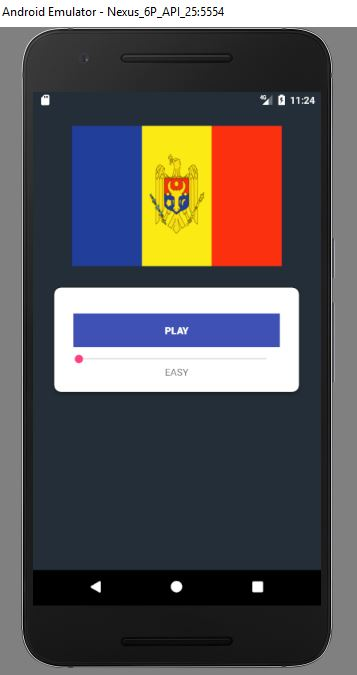
\includegraphics[width=0.5\textwidth]{Cattura.JPG}
	
	\caption{Deschiderea aplicatiei}
	
	\label{Im_label}
	
\end{figure}

\begin{figure}[!ht]
	
	\centering
	
	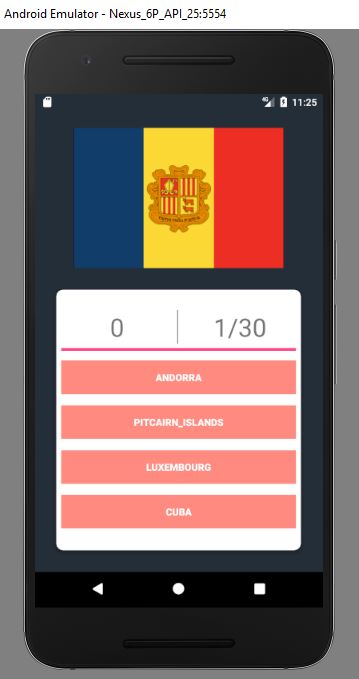
\includegraphics[width=0.5\textwidth]{Cattura1.JPG}
	
	\caption{Quiz-ul}
	
	\label{Im_label}
	
\end{figure}

\begin{figure}[!ht]
	
	\centering
	
	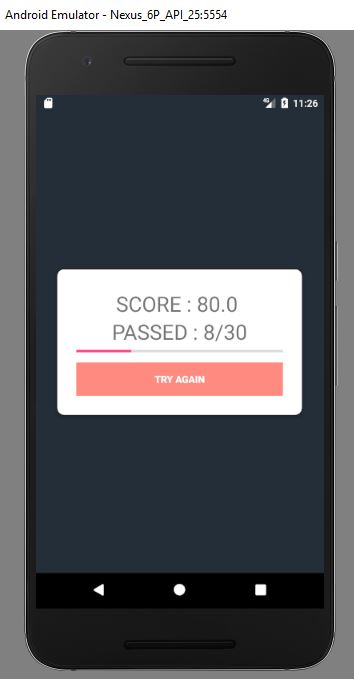
\includegraphics[width=0.5\textwidth]{Cattura2.JPG}
	
	\caption{Sfirsitul Quiz-ului}
	
	\label{Im_label}
	
\end{figure}


\clearpage